%%%%%%%%%%%%%%%%%%%%%%%%%%%%%%%%%%%%%%%%%%%%%%%%%%%%%%%%%%%%%%%%%%%%%%%%
%    INSTITUTE OF PHYSICS PUBLISHING                                   %
%                                                                      %
%   `Preparing an article for publication in an Institute of Physics   %
%    Publishing journal using LaTeX'                                   %
%                                                                      %
%    LaTeX source code `ioplau2e.tex' used to generate `author         %
%    guidelines', the documentation explaining and demonstrating use   %
%    of the Institute of Physics Publishing LaTeX preprint files       %
%    `iopart.cls, iopart12.clo and iopart10.clo'.                      %
%                                                                      %
%    `ioplau2e.tex' itself uses LaTeX with `iopart.cls'                %
%                                                                      %
%%%%%%%%%%%%%%%%%%%%%%%%%%%%%%%%%%
%
%
% First we have a character check
%
% ! exclamation mark    " double quote  
% # hash                ` opening quote (grave)
% & ampersand           ' closing quote (acute)
% $ dollar              % percent       
% ( open parenthesis    ) close paren.  
% - hyphen              = equals sign
% | vertical bar        ~ tilde         
% @ at sign             _ underscore
% { open curly brace    } close curly   
% [ open square         ] close square bracket
% + plus sign           ; semi-colon    
% * asterisk            : colon
% < open angle bracket  > close angle   
% , comma               . full stop
% ? question mark       / forward slash 
% \ backslash           ^ circumflex
%
% ABCDEFGHIJKLMNOPQRSTUVWXYZ 
% abcdefghijklmnopqrstuvwxyz 
% 1234567890
%
%%%%%%%%%%%%%%%%%%%%%%%%%%%%%%%%%%%%%%%%%%%%%%%%%%%%%%%%%%%%%%%%%%%
%

%AIP Reprint Class%%%%%%%%%%%%%%%%%%%%%%%%%%%%%%%%%%%%%%%%%%%%%%%%%%%%%%%%%%%%%%%%%%%%%%%%%%%%%
\documentclass[aip,prl,amsmath,amssymb,reprint,superscriptaddress]{revtex4-1} %preprint version
\usepackage{graphicx}% Include figure files
\usepackage{dcolumn}% Align table columns on decimal point
\usepackage{bm}% bold math
\usepackage{epstopdf}

    \renewcommand{\topfraction}{0.9}    % max fraction of floats at top
    \renewcommand{\bottomfraction}{0.8}    % max fraction of floats at bottom
    \setcounter{topnumber}{2}
    \setcounter{bottomnumber}{2}
    \setcounter{totalnumber}{4}     % 2 may work better
    \setcounter{dbltopnumber}{2}    % for 2-column pages
    \renewcommand{\dbltopfraction}{0.9}    % fit big float above 2-col. text
    \renewcommand{\textfraction}{0.07}    % allow minimal text w. figs
    \renewcommand{\floatpagefraction}{0.7}    % require fuller float pages
    \renewcommand{\dblfloatpagefraction}{0.7}    % require fuller float pages
    \setlength{\abovecaptionskip}{5pt}
    \setlength{\belowcaptionskip}{5pt}
    \setlength{\parskip}{0pt}
    \setlength{\textfloatsep}{5pt} 

%%%%%%%%%%%%%%%%%%%%%%%%%%%%%%%%%%%%%%%%%%%%%%%%%%%%%%%%%%%%%%%%%%%%%%%%%%%%%%%%%%%%%%%%%%%%%%%%%%

%IOP preprint class %%%%%%%%%%%%%%%%%%%%%%%%%%%%%%%%%%%%%%%%%%%%%%%%%%%%%%%%%%%%%%%%%%%%%%%%%%%%%%
%\documentclass[12pt]{iopart}
%\newcommand{\gguide}{{\it Preparing graphics for IOP journals}}
%Uncomment next line if AMS fonts required
%\usepackage{iopams}
%\usepackage{graphicx}
%\usepackage{epstopdf}  
%%%%%%%%%%%%%%%%%%%%%%%%%%%%%%%%%%%%%%%%%%%%%%%%%%%%%%%%%%%%%%%%%%%%%%%%%%%%%%%%%%%%%%%%%%%%%%%%%%
%Slava's inserts %%%%%%%%%%%%%%%%%%%%%%%%%%%%%%%%%%%%%%%%%%%%%%%%%%%%%%%%%%%%%%%%%%%%%%%%%%%%%%
%\usepackage{amsfonts}
%\usepackage{amssymb}

%\newcommand{\ptt}[1]{\frac{\partial#1}{\partial t}}
%\newcommand{\vvec}{\mathbf{v}}
%\newcommand{\Bvec}{\mathbf{B}}
%\newcommand{\Evec}{\mathbf{E}}
%\newcommand{\Jvec}{\mathbf{J}}
%\newcommand{\Avec}{\mathbf{A}}
%%%%%%%%%%%%%%%%%%%%%%%%%%%%%%%%%%%%%%%%%%%%%%%%%%%%%%%%%%%%%%%%%%%%%%%%%%%%%%%%%%%%%%%%%%%%%%%%%%

\begin{document}
\title{Spatial correlations in a turbulent MHD laboratory plasma}

\author{A. Wan}
\affiliation{Swarthmore College, Swarthmore, PA, USA}
\author{D.A. Schaffner}
\affiliation{Swarthmore College, Swarthmore, PA, USA}
\author{V.S. Lukin}
\affiliation{Space Science Division, Naval Research Laboratory, Washington, DC, USA}
\author{W.H. Matthaeus}
\affiliation{Bartol Research Institute and Department of Physics and Astronomy, University of Deleware, Newark, DE, USA}
\author{M.R. Brown}
\affiliation{Swarthmore College, Swarthmore, PA, USA}
\date{\today}
\begin{abstract}
Correlation analysis is used to determine the Taylor microscale and magnetic Reynold's number in a turbulent laboratory MHD plasma.  We find that radial correlation length is shorter for a colliding MHD wind tunnel plasma than for a single plume.  An unambiguous measure of the magnetic Reynolds number is estimated from the Taylor microscale and the correlation scale, then compared to a calculation using the Spitzer resistivity.
\end{abstract}

\maketitle

\section{Introduction}

A useful measure of fully developed turbulence is the spatial correlation function.  For a magnetohydrodynamic (MHD) plasma, the radial correlation function of the magnetic field can be written
%
\begin{equation}
R(r) =  \langle {\bf b(x) \cdot b(x + r)} \rangle
\label{eq:correlation1}
\end{equation}
%
where {\bf b} is the fluctuating part of a turbulent magnetic field (${\bf B}(x, t) = {\bf B_0 + b}$).  For well-behaved turbulence, the magnetic fluctuations at two points should become uncorrelated at large spatial separation and the correlation function should vanish ($R \rightarrow 0$ as $r \rightarrow \infty$).  

Two point velocity correlation functions have been measured in conventional fluids for decades (see, for example \cite{frisch95}) but two point magnetic correlations in plasmas are less common.  The first proper two-point single time measurements of the magnetic correlation function in the solar wind plasma were performed by Matthaeus, et al \cite{Matthaeus05}.  They used simultaneous magnetic field data from several spacecraft, including the four Cluster spacecraft flying in tetrahedral formation.  Simultaneous measurements were performed with separations ranging from $150~km$ (using pairs of Cluster satellites) to $350~R_E$ ($2.2 \times 10^6~km$).  From measurements of the outer correlation scale, and the Taylor microscale (discussed below), they report an effective magnetic Reynolds number of the solar wind $R_m^{eff}  = 230,000$.

In a set of follow-up papers, Weygand, et al \cite{Weygand07,Weygand09,Weygand10,Weygand11} have modified and improved the earlier result.  In particular, they describe a method using fits of Cluster separations from 100 to $10^6~km$ \cite{Weygand07}, and extrapolating the Taylor microscale down to zero separation.  We discuss this method below.  These more detailed measurements confirm the earlier work  \cite{Matthaeus05} and find a solar wind magnetic Reynolds number of $R_m^{eff}  = 260,000 \pm 20,000$.  In addition, using data in the magnetospheric plasma sheet (tailward of Earth), they find a much smaller Reynolds number $R_m^{eff}  = 111 \pm 12$ since the outer correlation scale is much smaller in the plasma sheet.  Anisotropies in the correlation function parallel and perpendicular to the local magnetic field were studied in separate papers \cite{Weygand09,Weygand10}, with longer correlation lengths measured parallel to the local field.  Variations with solar wind speed were also studied \cite{Weygand11}.

%\begin{figure}[!htbp]
%\centerline{
%\includegraphics[width=8.5cm]{helicity_scaling.png}}
%\caption{\label{fig:helicity_scaling} (a) Average magnetic field magnitude over the equilibrium epoch (40-60$\mu s$), (b) injected gun energy and volume integrated magnetic field energy, and (c) amount of helicity injected in the first $20 \mu s$ after discharge trigger as a function of magnetic flux in gun core.}
%\end{figure}

\section{Theory and Techniques}

As noted above, the magnetic correlation function can be written
%
\begin{equation}
R(r) =  \langle {\bf b(x) \cdot b(x + r)} \rangle
\end{equation}
%
where {\bf b} is the fluctuating part of a turbulent magnetic field (${\bf B}(x, t) = {\bf B_0 + b}$). 

The magnetic Taylor microscale can be formally defined as
%
\begin{equation}
\lambda_T^2 = \frac{\langle {\bf b}^2 \rangle}{\langle (\nabla \times {\bf b})^2 \rangle}.
\label{eq:tayscale}
\end{equation}
%
This definition identifies the Taylor microscale as the scale associated with mean square spatial derivatives of the fluctuating magnetic field $\bf{b}$. A similar definition of the Taylor microscale in conventional fluids involves spatial derivatives of the fluctuating velocity field \cite{frisch95}. It is at this scale that one would expect dissipation effects to become important, although actual dissipation likely occurs at smaller, kinetic scales ($k_D \lambda_T = R_m^{1/4}$) \cite{Matthaeus08}.  We expect that the Taylor microscale should be on the order of but larger than the Larmor scale ($\rho_i \approx 1~mm$ in the SSX wind tunnel) and the ion inertial scale ($c/\omega_{pi} \approx 5~mm$ in SSX).

The correlation scale can be evaluated
%
\begin{equation}
\lambda_{C}  = \frac{1}{\langle b^2 \rangle} \int_0^\infty R(r) dr
\label{eq:tayscale2}
\end{equation}
%
which is of the order of the system size (eg. the radius of the SSX wind tunnel).

An equivalent formulation of the Taylor scale in terms of the spectrum is
%
\begin{equation}
\frac{1}{\lambda_T^2}  = \int_0^\infty dk k^2 E(k)/\int_0^\infty dk E(k)
\label{eq:tayscale3}
\end{equation}
%
The correlation function can be approximated
\begin{equation}
R(r) \approx  \langle b^2 \rangle \left(1 - \frac{r^2}{2 \lambda_T^2}  \right)
\label{eq:correlation2}  
\end{equation}
%
We will fit our measured 16-point correlation function $R(r)$ to this form in order to extract the Taylor microscale $\lambda_T$. 

An effective turbulent magnetic Reynolds number can be written \cite{frisch95}
%
\begin{equation}
R_m^{eff}  = \left(\frac{\lambda_{C}}{\lambda_T} \right)^2
\label{eq:RM-eff}
\end{equation}
%
which is related to the actual magnetic Reynolds number
%
\begin{equation}
R_m  = \left( R_m^{eff} \right) ^2 .
\label{eq:RM-eff2}
\end{equation}
%
Note that the formal definition of the magnetic Reynolds number involves the plasma (Spitzer) conductivity
\begin{equation}
R_m = \mu_0 V \sigma_{SP} L.
\label{eq:RM-calc} 
\end{equation}
%
Using $T_e = 10~eV$ for the SSX wind tunnel and the radius of the tunnel for the outer scale ($L = R = 0.078~m$), we calculate $R_m = 300$ for a flow speed of 50 km/s.

The Fourier transform of the correlation function is the spatial energy spectrum, $E(k)$:
%
\begin{equation}
E(k) = \frac{1}{2 \pi} \int_0^L e^{ikr} R(r) dr
\label{eq:spectrum1}
\end{equation}
%
We can compare a measurement of the energy spectrum $E(k)$ to the Fourier transform of the measured correlation function $R(r)$.

\section{Experimental Apparatus}

\begin{figure}[!htbp]
\centerline{
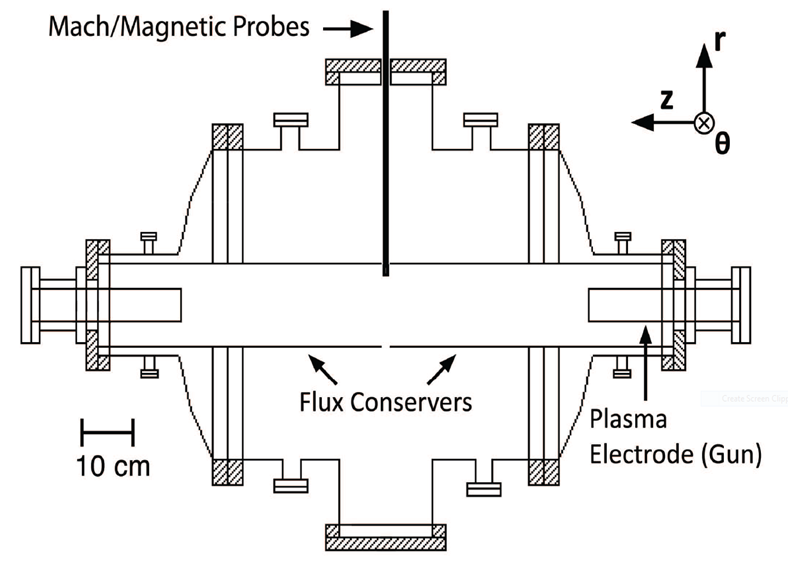
\includegraphics[width=8.5cm]{Images/chamberEdit.png}}
\caption{\label{fig:chamber} Cross-section of SSX chamber in MHD wind-tunnel configuration}
\end{figure}

\textsf{TODO: Need some standard experiment setup description. Plasma production, lab info? Definitely need to talk about the magnetic probes: tri-directional $\dot{B}$ probes inserted radially at the mid-plane of the flux conserver. Measures change in magnetic field at 16 points along radius.}

The SSX operates in two configurations, relaxation and merging. In the relaxation configuration one plasma gun is fired and the relaxation of the plasma plume (\textsf{reference the Taylor relaxation paper}) is observed. In the merging configuration, two plasmas with opposing helicities are created and their subsequent interaction is studied.

bla

bla

bla

\section{Results}

Fig.\ \ref{fig:brbtbz} shows the averaged autocorrelation function for integrated $B$-field in each of the three probe directions. 75 runs of the single-plume relaxation configuration were sampled, the $40.0-60.0\ \mu s$ epoch being used in each case. The darkened data points indicate which points were used in plotting the fit equation \eqref{eq:correlation2}. Each distinct point represents a correlation measured from a given probe tip: thus there are $16-n$ points for a $n$ tip separation. Apart from providing a visual representation of experimental spread in data, this method also reveals locational variations in the correlation function that persist over multiple shots. For example, in Fig.\ \ref{fig:brbtbz}(b), it appears that there are two clusters of data, one with a generally higher correlation strength than the other. The higher correlation strength points correspond to tips further from the wall of the flux conserver; that this pattern is apparent after an averaging of 75 sets of data suggests that $B_\theta$ correlation strengths are influenced by wall proximity. Fig.\ \ref{fig:brbtbz}(b) shows how the parabolic fit \eqref{eq:RM-eff} can be applied to a subset of the data --- in this case the fit shown was performed only on the averaged correlation strengths from the four outer probe tips.

Fig.\ \ref{fig:brbtbz} provides an enlightening contrast between the three measured directions of magnetic field. The $B_r$ field is highly correlated throughout, while in contrast the $B_z$ correlation strengths are highly scattered and less suggestive of any distinctive pattern. As such, it is prudent to focus on the correlation strengths of the $B_\theta$ signal, which are well-clustered and exhibit a sharper decay in correlation strength, thus giving a more precise measurement of the Taylor microscale $\lambda_T$. We proceeded to compare the correlation strengths of $B_\theta$ from merging and relaxation configurations of SSX with corresponding simulations. 

\begin{figure}[!htbp]
\centerline{
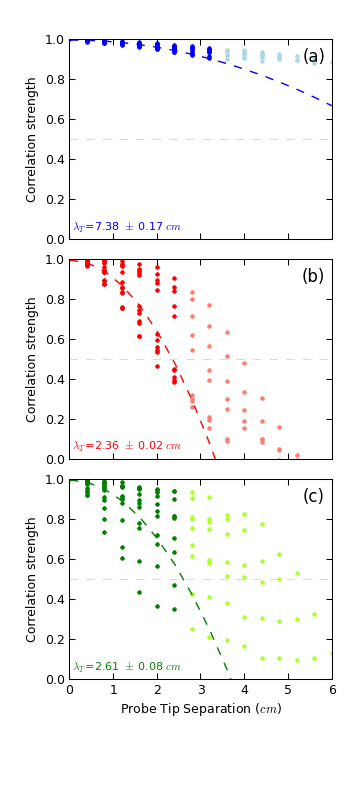
\includegraphics[width=8.5cm]{Images/brbtbz-081413.png}}
\caption{Single plume correlation functions for magnetic field in the (a) $\hat{r}$, (b) $\hat{\theta}$, (c) $\hat{z}$ directions}
\label{fig:brbtbz}
\end{figure}

\textsf{TODO get Slava's description here? Relevant details such as the paradigm used (Hall/MHD), etc...}
The simulation data consisted of magnetic field measured along 8 equally-spaced radii at the midplane of the simulated flux conserver. 

The simulation epoch used was $43-53 \mu s$, chosen to capture fluctuations in the simulated $B$-field that qualitatively resembled the $40-60\ \mu s$ epoch of the experimental data. \textsf{TODO: need to try different epochs of the simulation data.}

Fig.\ \ref{fig:comparisons} compares the measured auto-correlation functions from merging and relaxation configurations of the experiment and of simulation. Fig.\ \ref{fig:comparisons}(a) presents the results from the two configurations of SSX, namely single plume (relaxation) and merging. The steeper decay of the merging configuration correlation function is indicative of a more turbulent plasma during the sampled epoch, which is intuitively expected.

The curves in Fig.\ \ref{fig:comparisons}(b) correspond to the relaxation configuration for SSX and simulation. 
While the two correlation curves look qualitatively different, it is enlightening that the radii of curvature (i.e.\ the curve obtained by fitting \eqref{eq:RM-eff}) obtained from experiment and from simulation are close. \textsf{mini-conclusion?} 

Fig.\ \ref{fig:comparisons}(c) presents results from the merging configuration in SSX and simulation. 
The contrast between the laboratory and simulated results motivates deeper consideration of details of the simulation that differ from an experimental setup. One potential source of differences between the two is that the simulated plasmas always merge exactly at the midplane, and thus exactly where the measurements of $B$-field are obtained. Using measurements slightly offset from the midplane of the simulation could imitate the variability in the merging plane of lab plasmas.

\begin{figure}[!htbp]
\centering
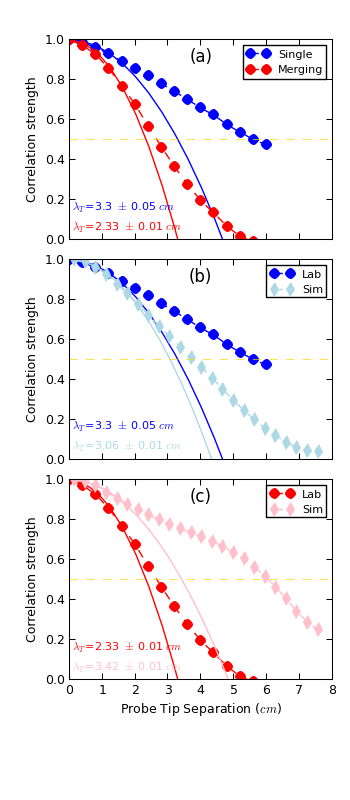
\includegraphics[width=8.5cm]{Images/comparisons.png}
\caption{\label{fig:comparisons} (a) Single vs.\ Merging. (b) Single, Lab vs.\ Sim. (c) Merging, Lab vs.\ Sim.}
\end{figure}

As shown in Figures \ref{fig:brbtbz} and \ref{fig:comparisons}, \eqref{eq:RM-eff} can be fitted to functions of correlation strength to obtain a value for the Taylor microscale $\lambda_T$. 
Following the example of Matthaeus et al.\cite{Matthaeus05}, we vary the degrees of freedom given in fitting \eqref{eq:RM-eff} to the data and extrapolate to a zero-point fit. This theoretically corresponds to the infinitesimal measurement of the correlation function's radius of curvature, and thus to the most physically accurate value of the Taylor microscale $\lambda_T$. 
(\textsf{TODO check the corresponding section in Bill's paper and use their language}) 

\begin{figure}[!htbp]
\centerline{
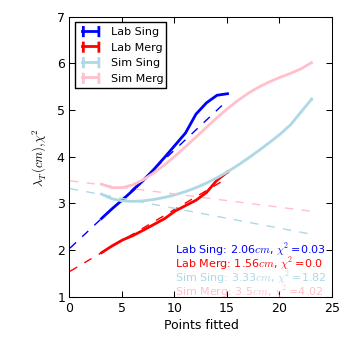
\includegraphics[width=0.5\textwidth]{Images/ndf.png}}
\caption{\label{fig:ndf} $\lambda_T$ vs. ndf. of parabola fit with error}
\end{figure}

Fig.\ \ref{fig:ndf} corresponds to Fig.\ BLAH in \cite{Matthaeus05}, and shows the results of extrapolating the measured $\lambda_T$ values to a zero-point fit. The simulation data show a curious inflection at points fitted $\sim 5$, which could be caused by BLAH. The laboratory results, however, fit well to a linear function and yield well-defined values of the Taylor microscale: $\lambda_T = 2.06cm$ for the relaxation configuration, and $\lambda_T = 1.56cm$ for the merging setup. 

Once this extrapolated $\lambda_T$ value has been obtained, calculating $R_m$ requires a measurement of the correlation length $\lambda_C$. A variety of ways exist for calculating $\lambda_C$, which is the fundamental length scale of the experiment: the radius of the flux conserver is a natural maximum length scale for radial correlation measurements; fitting the fitted correlation function to a Gaussian yields an integration scale or an $e$-folding time. 

\textsf{Sample calculation of $R_m$ values: ``w/ radius'' means using $\lambda_C = 7.8\ cm$ (?), ``w/ Int. Scale'' means performing the fit to find e-folding time (Talk about measuring correlation length: Gaussian/other fits), computed means using the formula for $R_m$ with Spitzer resistivity. Hopefully they all end up in the same ballpark. }

Table \ref{tab:Rms} compares the magnetic Reynolds numbers obtained from four different data sets: experimental single-plume and merging configurations, and their corresponding simulations. It compares the values of $R_m$ obtained when the various $\lambda_C$ calculations are performed: the ``$R_m$ w/ Radius'' column uses the radius of the flux chamber as the correlation scale, $\lambda_C = 7.8\ cm$; the ``w/ Int. Scale'' performs the integration in \eqref{eq:tayscale2} to calculate the correlation scale. 

These results are comparable to the magnetic Reynolds number calculated using \eqref{eq:RM-calc}, $R_M = 300$. 

Any uncertainty in fitting \eqref{eq:correlation2} to the data is magnified when the ratio $\lambda_C/\lambda_T$ is raised to the fourth power. An estimate of the error in the Lab Single value of $R_m$ calculated using the radius is 
%
\begin{equation}
\Delta R_m = 4 (\dfrac{\Delta \lambda_T}{\lambda_T} + \dfrac{\Delta \lambda_C}{\lambda_C}) = 4 (\dfrac{0.054}{3.30} + \dfrac{0.1}{7.8})= 11.7\%
\label{eq:error}
\end{equation}
%
\textsf{TODO is this the right way to estimate error?}

\begin{table} [htbp]
\caption{\label{tab:Rms}Comparison of measured/computed Taylor Microscale and magnetic Reynolds numbers for various cases.}
\begin{tabular}{|r|c|c|c|}
\hline
Condition& $\lambda_{T}$&$R_{m}$ w/Radius&$R_{m}$ w/Int. Scale\\
\hline
Lab Single  & 2.06 & 206 & -1\\
Sim Single  & 3.33 & 30.1 & -1\\
Lab Merging & 1.56 & 625 & -1\\
Sim Merging & 3.50 & 24.7 & -1\\
\hline
\end{tabular}
\end{table}

The values obtained for the two configurations in the laboratory straddle the value of $R_m$ calculated from \eqref{eq:RM-calc}. This agreement (check error?) is BLAH --- \textsf{Something about how this method is cool because we were able to obtain a value for two physical parameters ($\lambda_T$ and $R_m$) just through a correlation analysis, which basically looks at turbulence/noise? Plus this method is useful for plasmas that we can't directly measure temperature for --- good alternative to the calculation with Spitzer resistivity.}


% ----------------------------------------------------------------
\section*{Acknowledgements}
We gratefully acknowledge many useful discussions with William Matthaeus. This work has been funded by the US DoE Experimental Plasma Research program and the National Science Foundation.  The simulations were performed using the advanced computing resources (Cray XC30 Edison system) at the National Energy Research Scientific Computing Center.
% ----------------------------------------------------------------
\section*{References}
\begin{thebibliography}{99}

%\bibitem{Belmabrouk98}
%Belmabrouk, H., and M. Michard (1998), Taylor length scale measurement by laser Doppler velocimetry, Exp. Fluids, 25, 69Ð76.

\bibitem{Matthaeus05}
Matthaeus, W. H. and Dasso, S. and Weygand, J. M. and Milano, L. J. and Smith, C. W. and Kivelson, M. G., Phys. Rev. Lett. 95, 231101 (2005) Spatial Correlation of Solar-Wind Turbulence from Two-Point Measurements

\bibitem{Weygand07}
Weygand, J. M., Matthaeus, W. H., Dasso, S., Kivelson, M. G.,
and Walker, R. J. (2007), J. Geophys. Res., 112, A10201.

\bibitem{Weygand09}
Weygand, J. M., Matthaeus, W. H., Dasso, S., Kivelson, M. G.,
Kristler, L. M., and Mouikis, C. (2009), J. Geophys. Res., 114,
A07213.

\bibitem{Weygand10}
Weygand, J. M., Matthaeus, W. H., El-Alaoui, M., Dasso, S., and
Kivelson, M. G. (2010), J. Geophys. Res., textit115, A12250.

\bibitem{Weygand11}
Weygand, J. M., Matthaeus, W. H., Dasso, S., and Kivelson, M.
G. (2011), J. Geophys. Res., 116, A08120.

\bibitem{Matthaeus08}
Matthaeus W. H., Weygand, J. M., Chuychai, P., Dasso, S.,
Smith, C. W., and Kivelson, M. (2008), Astrophys. J., 678,
L141.

\bibitem{frisch95}Frisch, U. 1995, {\it Turbulence} (Cambridge: Cambridge Univ. Press)

%\bibitem{sorrisovalvo99}Sorriso-Valvo, L. {\it et al.} Geophys. Res. Lett. {\bf 26}, 1801–1804 (1999).

%\bibitem{wan12}Wan, M. {\it et al.} ApJ. {\bf 744} 177 (2012).

%\bibitem{sorrisovalvo01}Sorriso-Valvo, L. {\it et al.} Planet. Space Sci. {\bf 49}, 1193–1200 (2001).

%\bibitem{marrelli05}Marrelli, L. {\it et al.} Phys. Plasmas. {\bf 12}, 030701 (2005).

%\bibitem{Greco08}A. Greco, P. Chuychai, W. H. Matthaeus, S. Servidio and P. Dmitruk, Intermittent MHD structures and classical discontinuities, Geophys. Res. Lett. {\bf 35}, L19111 (2008).

%\bibitem{Greco09}Greco, A., Matthaeus, W. H., Servidio, S., Chuychai, P., and Dmitruk, P.: Statistical Analysis of Discontinuities in Solar Wind ACE Data and Comparison with Intermittent MHD Turbulence, ApJ {\bf 691}, L111 (2009).

%\bibitem{Wan09}Wan, M., Oughton, S., Servidio, S., and Matthaeus, W. H.: Generation of non-Gaussian statistics and coherent structures in ideal magnetohydrodynamics, Phys. Plasmas {\bf 16}, 080703 (2009).

%\bibitem{Servidio11b}Servidio, S. {\it et al}, J. Geophys. Res. {\bf 116}, A09102 (2011).

%\bibitem{Gray13} T. Gray, M. R. Brown, and D. Dandurand. Phys. Rev. Lett. {\bf 110}, 085002 (2013). 

%\bibitem{schaffner14} D.A. Schaffner {\it et al.} Turbulence analysis of an experimental flux rope plasma. Submitted to Plas. Phys. Cont. Fusion. (2014).

%\bibitem{Taylor86} J. B. Taylor, Rev. Mod. Phys. {\bf 58}, 741 (1986).

%\bibitem{Matthaeus80} W.H. Matthaeus and D. Montgomery, Ann. N.Y. Acad. Sci. {\bf 357}, 203 (1980).

%\bibitem{torrence98}C. Torrence, G.P. Compo, A practical guide to wavelet analysis. Bull. Am. Meteorol. Soc. {\bf 79}, 6178 (1998).

%\bibitem{clauset09}A. Clauset, C. Rohilla Shalizi, M.E.J. Newman, Power-law distributions in empirical data, SIAM Rev. {\bf 51}, 661703 (2009).

%\bibitem{wan12}M. Wan, K. T. Osman, W. H. Matthaeus, and S. Oughton, Investigation of intermittency in magnetohydrodynamics and solar wind turbulence: scale-dependent kurtosis, ApJ {\bf 744}, 171 (2012).

%\bibitem{Gray10}T. Gray, V. S. Lukin, M. R. Brown, C. D. Cothran, Three-dimensional reconnection and relaxation of merging spheromak plasmas, Phys. Plasmas {\bf 17}, 102106 (2010).

%\bibitem{goldstein94}Goldstein, M.L., Roberts, D.A. and Fitch, C.A. Jour. Geo. Res. {\bf 99} 11519-11538 (1994).

%\bibitem{ji95}Ji, H., Prager, S.C. and Sarff, J.S. Phys. Rev. Lett. {\bf 74} 2945 (1995).

%\bibitem{telloni12}Telloini, D. {\it et al.}. ApJ. {\bf 751} 19 (2012).

%\bibitem{matthaeusVelli11}Matthaeus, W.H. and Velli, M. Space Sci. Rev. {\bf 160} 145-168 (2011).

%\bibitem{greco12}A. Greco {\it et al.} ApJ. {\bf 749} 105 (2012).

\end{thebibliography}

\end{document}

